\chapter{Discussion}

\fancyhead[L]{Chapter 4: Discussion}
\fancyfoot[C]{\thepage}

\section{Influence of External Parameters on\\ Initial Conditions}
The results indicate that external parameters significantly influence the system's initial state. 
By "initial conditions," we refer to the system properties immediately after introducing external inputs, including changes in density, temperature, and composition.

External inputs modify the overall density due to differences in intrinsic properties (e.g., phase or composition) between the introduced component and the existing system. Similarly, energy transfer between components can result in temperature changes governed by conservation of energy principles. These coupled effects establish the foundation for subsequent system behavior and performance.

The interplay of these factors—density, temperature, and energy distribution—is critical in shaping the observed outcomes. Below, we analyze how variations in external parameters drive system dynamics across different scenarios.

\begin{figure}[h!]
    \centering
    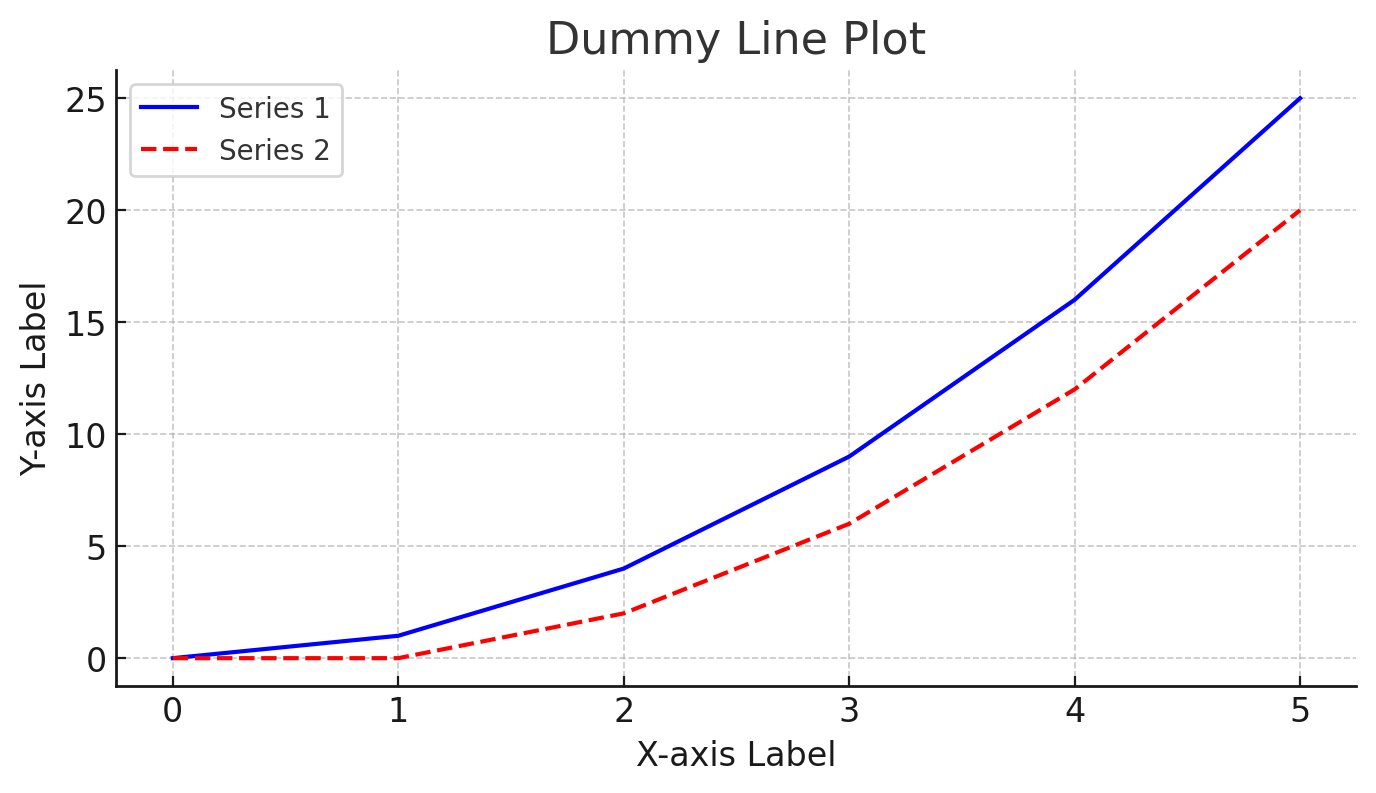
\includegraphics[width=130mm,scale=0.6]{body/images/placeholder_image1.png}
    \caption[System Properties at Initial State]{Example plot showing variations in density and temperature as a function of external input.}
    \label{fig:initial_conditions}
\end{figure}

\section{System Behavior Across Parameter Space}
The system exhibits distinct behaviors under varying external input conditions, which we classify into four broad regions based on performance metrics.

\subsection*{Region 1: Stable Performance}
At low input levels, the system remains close to baseline conditions, with minimal deviations observed in output parameters such as velocity, energy efficiency, or system height. These stable dynamics suggest that the system's resilience to external changes is high in this range.

\begin{figure}[h!]
    \centering
    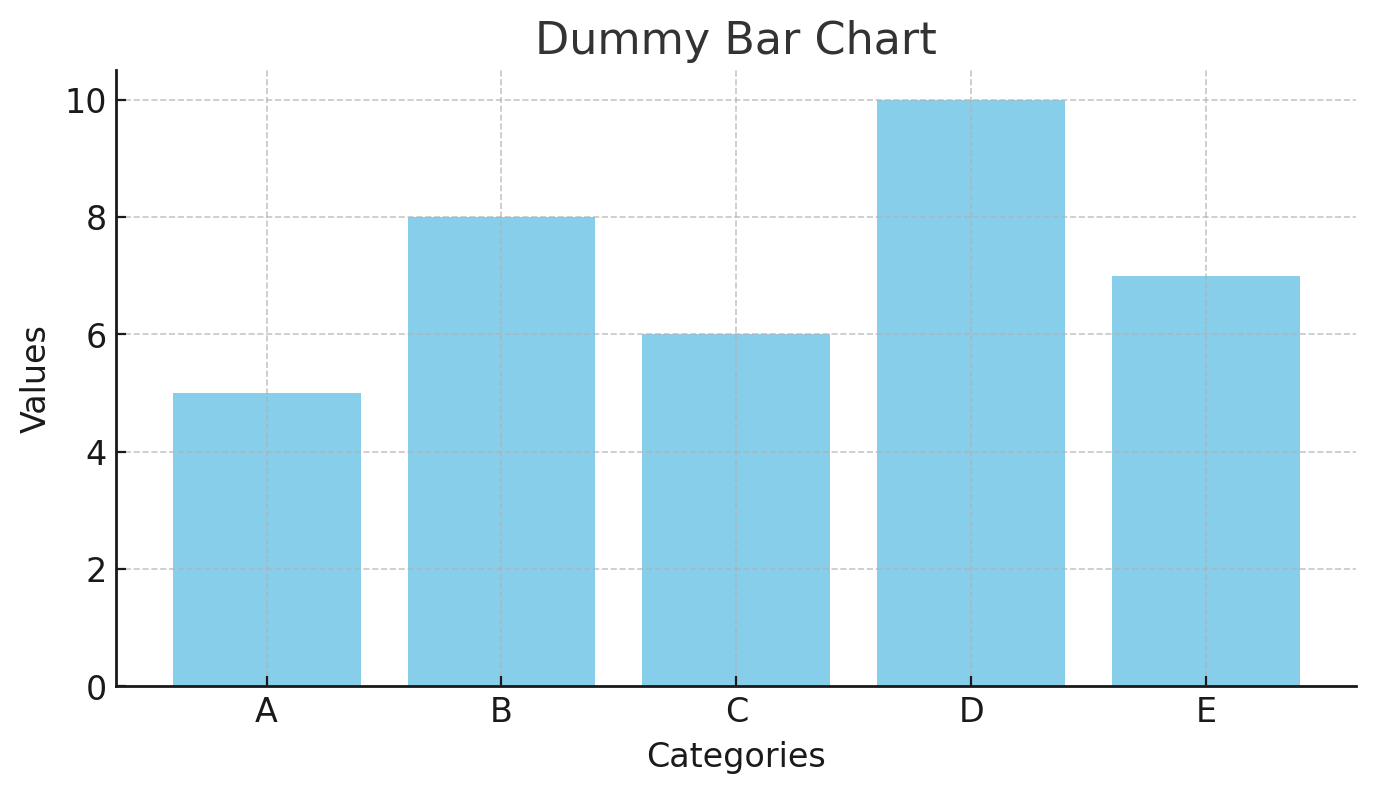
\includegraphics[width=130mm,scale=0.6]{body/images/placeholder_image2.png}
    \caption[Stable Dynamics]{Sample results showing minimal impact of external inputs on system behavior in Region 1.}
    \label{fig:region1_plot}
\end{figure}

\subsection*{Region 2: Performance Suppression}
At moderate input levels, external parameters begin to significantly suppress system performance. Key metrics, such as energy efficiency or output rate, decline due to increased resistance or diminished energy availability. This behavior reflects the onset of critical thresholds beyond which system capacity is constrained.

\begin{figure}[h!]
    \centering
    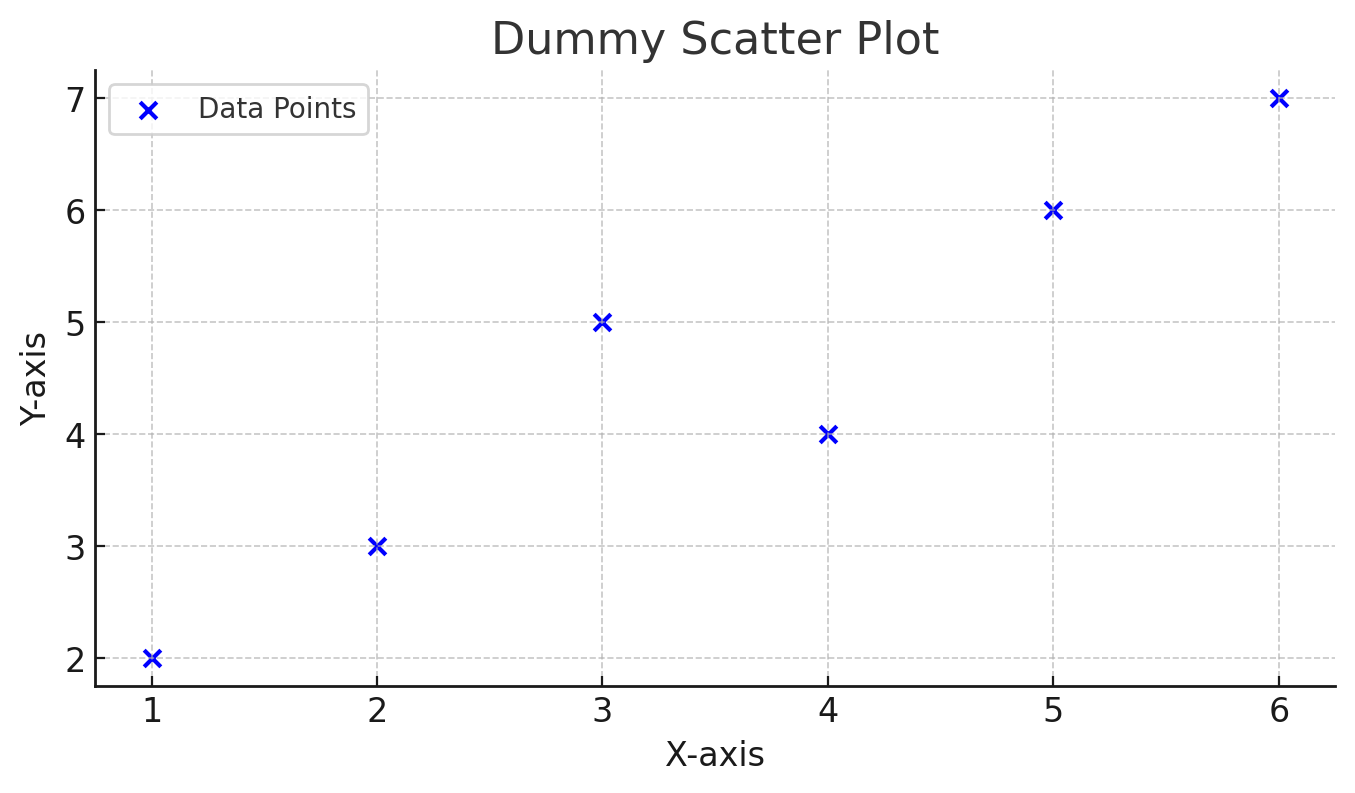
\includegraphics[width=130mm,scale=0.6]{body/images/placeholder_image3.png}
    \caption[Suppressed Dynamics]{Sample results showing significant suppression of system output due to moderate external inputs in Region 2.}
    \label{fig:region2_plot}
\end{figure}


\section{Comparison to Observational Data}
To validate key findings, model results were compared to observational data from analogous systems. The comparison reveals broad alignment in trends but also highlights discrepancies in specific cases, particularly at extreme input levels. These discrepancies underscore the need for refined assumptions or additional factors in the model.

\begin{figure}[h!]
    \centering
    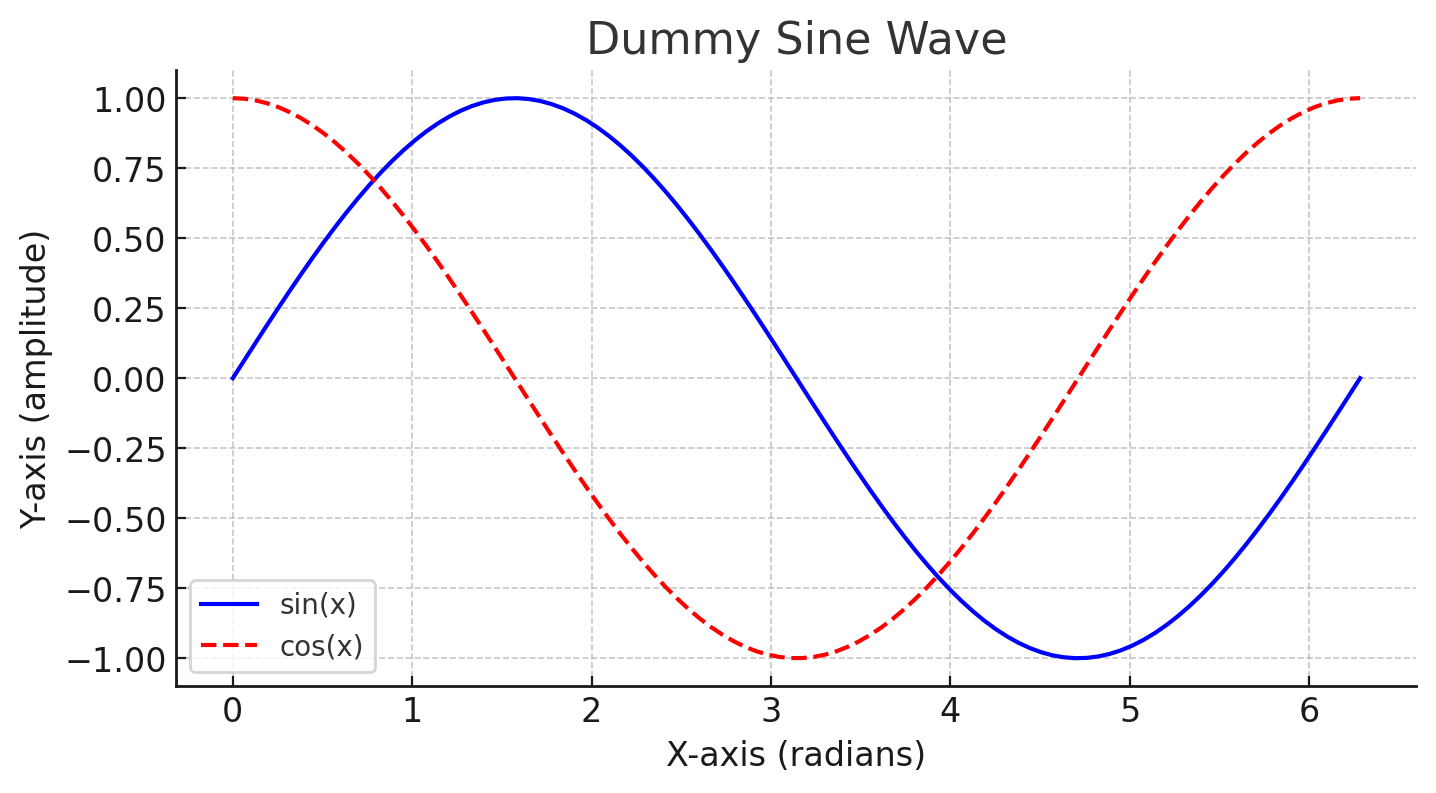
\includegraphics[width=150mm,scale=0.9]{body/images/placeholder_image4.png}
    \caption[Model vs Observations]{Comparison of model predictions with observational data. Shaded regions indicate areas of divergence.}
    \label{fig:model_vs_observations}
\end{figure}

\subsection*{Case Study A}
One observed system closely matched the model's predictions, supporting the robustness of the underlying assumptions. Minor deviations were attributed to environmental variability.

\subsection*{Case Study B}
Another case revealed significant deviations, suggesting the presence of unmodeled interactions or system complexities. These results highlight opportunities for further model refinement.

\section{Implications and Future Research}
The findings have broad implications for understanding system dynamics and optimizing performance.

Future research should aim to address identified model limitations, incorporate additional variables, and extend validation efforts using experimental or field data.

\section{Conclusion}
This discussion highlights the significant influence of external parameters on system dynamics. By analyzing distinct performance regions and comparing results to observations, we gain valuable insights into system behavior. These findings form a foundation for future work aimed at refining models and improving predictive accuracy.
